\section{Problema I}
Usando la Figura.1 como modelo, ilustre la operación de Insertion Sort en el arreglo $A = {31, 41, 59, 26, 41, 58}$.
    
    \begin{figure}[H]
    \centering
    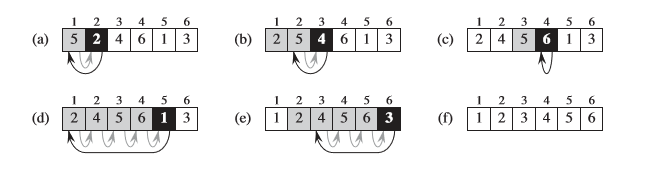
\includegraphics[width=0.5\textwidth]{img/fig1}
    \caption{Ilustración del algoritmo Insertion Sort}
    \label{fig1}
    \end{figure}

Siguiendo las instrucciones del algoritmo Insertion Sort para el arreglo especificado en el enunciado 1, se tiene el siguiente resultado:

    \begin{figure}[H]
    \centering
    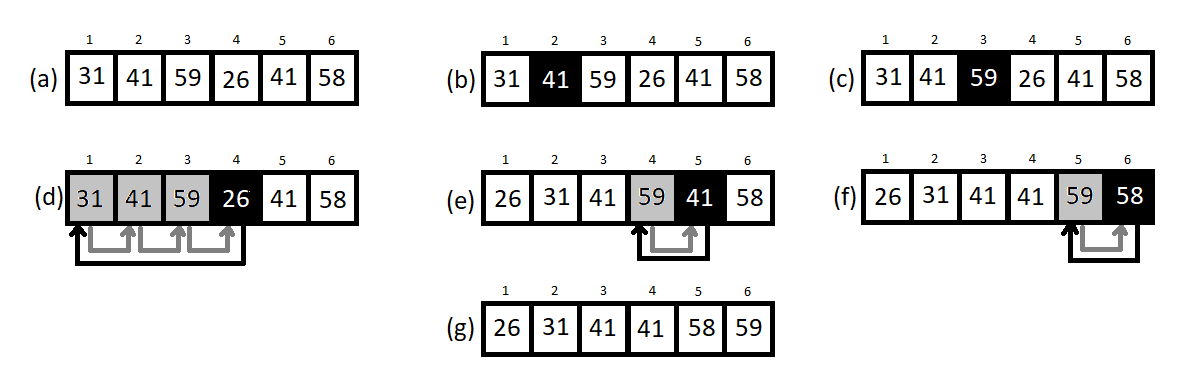
\includegraphics[width=0.5\textwidth]{img/fig2}
    \caption{Ilustración del algoritmo Insertion Sort para el arreglo del enunciado del problema I.}
    \label{fig2}
    \end{figure}
    
En la anterior figura se observa el proceso desde el arreglo inicial (Figura.2.a), hasta el arreglo resultante (Figura.2.g).